\onecolumn
\appendix

\noindent{\Large\bfseries Appendix}

\vspace{1.5em}
\noindent{\large\bfseries Table of Contents}
\vspace{0.5em}
\hrule
\vspace{1em}

\newcommand{\apptocmain}[3]{\noindent\textbf{#1}\hspace{1em}#2\dotfill\pageref{#3}\par\vspace{0.4em}}
\newcommand{\apptocsub}[3]{\noindent\hspace{2em}#1\hspace{0.8em}#2\dotfill\pageref{#3}\par\vspace{0.2em}}

\apptocmain{A}{\textbf{Prompts for Design, Control, and Judge Agents}}{app:prompts}
\apptocsub{A.1}{Design Agent Prompts}{app:design_prompts}
\apptocsub{A.2}{Control Agent Prompts}{app:control_prompts}
\apptocsub{A.3}{Judge Agent Prompts}{app:judge_prompts}
\vspace{0.2em}

\apptocmain{B}{\textbf{RL Training Hyperparameters}}{app:hyperparameters}

\apptocmain{C}{\textbf{Evaluation Budget}}{app:compute_budget}

\apptocmain{D}{\textbf{Reward Similarity and Example D2C Rewards}}{app:d2c_rewards}

\apptocmain{E}{\textbf{Baseline Implementation Details}}{app:baselines}

\apptocmain{F}{\textbf{Environment Details}}{app:environments}

\apptocmain{G}{\textbf{Additional Results}}{app:additional_results}
\apptocsub{G.1}{Statistical Significance Tests}{app:statistical_tests}
\apptocsub{G.2}{Critique-Action Correlation Analysis}{app:critique-analysis}
\apptocsub{G.3}{Example Debate Transcript}{app:debate-transcript}
\vspace{0.2em}

\apptocmain{H}{\textbf{Evaluation Metric Analysis}}{app:metric-correlation}

\apptocmain{I}{\textbf{LLM Backbone Sensitivity}}{app:llm-sensitivity}

\apptocmain{J}{\textbf{Open-Weight Backbone Analysis}}{app:open_weight_backbones}

\newpage

\section{Prompts}
\label{app:prompts}
\newcommand{\promptheading}[1]{\vspace{0.4em}\noindent\textbf{#1}\par}
\subsection{Design Agent}
\label{app:design_prompts}
Design-agent prompts are environment-specific. We show the Ant prompts below. Other environments follow the same structure with environment-specific parameter schemas and masked XML references.

\promptheading{Base system prompt.}
\begin{promptbox}
## Mission
Design a robot morphology optimized for the task: {task_description}

## Environment
The ant is a 3D quadruped robot with a central torso and four legs. Each leg consists of three segments connected by hinge joints: an attachment segment from torso to hip, a thigh segment, and a shin/ankle segment. The robot moves forward by coordinating torque across eight actuated joints (two per leg).

## Parameters
Output **exactly 10 strictly positive** parameters that define the robot structure. Any zero or negative value will invalidate the design and be rejected:

**Torso:**
- `param1`: Torso radius (spherical torso size)

**Leg Attachment Offsets** (relative to torso center):
- `param2`: X-offset for leg attachment point
- `param3`: Y-offset for leg attachment point

**Thigh Segment Direction** (from attachment point):
- `param4`: X-offset for thigh segment endpoint
- `param5`: Y-offset for thigh segment endpoint

**Shin/Ankle Segment Direction** (from thigh endpoint):
- `param6`: X-offset for shin/ankle segment endpoint
- `param7`: Y-offset for shin/ankle segment endpoint

**Capsule Radii:**
- `param8`: Hip/attachment segment capsule radius
- `param9`: Thigh segment capsule radius
- `param10`: Shin/ankle segment capsule radius

## Constraints
- Every parameter must be strictly positive. Even slight negatives (e.g., `-0.01`) or zeros break the MuJoCo XML generation, so ensure all values are > 0 before returning them.
- The four legs use symmetric parameter values (front/back and left/right mirrored). Provide the parameter magnitudes once; the XML generator handles the sign flips internally.

Explore broadly: avoid tiny perturbations of prior designs and feel free to propose meaningfully different morphologies while respecting the positivity and symmetry rules.
\end{promptbox}

\promptheading{Base user prompt.}
\begin{promptbox}
## Task
Design a robot morphology that can achieve the following task: {task_description}

## Context
Use any provided debate context to spot issues, but rely on your own judgment to propose a distinct morphology rather than small tweaks.

## Masked XML Reference
Use the masked MuJoCo XML snippet below to understand how the parameters populate the model:
"""
<mujoco model="ant">
  <compiler .../> <option .../> <default .../> <asset .../>
  <worldbody>
    ...
    <body name="torso" pos="0 0 {height}">
      <geom name="torso_geom" pos="0 0 0" size="{param1}" type="sphere"/>
      <joint name="root" type="free" .../>
      <!-- Front-left leg (other 3 legs use mirrored signs) -->
      <body name="front_left_leg" pos="0 0 0">
        <geom fromto="0 0 0 {param2} {param3} 0" size="{param8}" type="capsule"/>
        <body name="aux_1" pos="{param2} {param3} 0">
          <joint name="hip_1" type="hinge" range="-40 40" .../>
          <geom fromto="0 0 0 {param4} {param5} 0" size="{param9}" type="capsule"/>
          <body pos="{param4} {param5} 0">
            <joint name="ankle_1" type="hinge" range="30 100" .../>
            <geom fromto="0 0 0 {param6} {param7} 0" size="{param10}" type="capsule"/>
          </body>
        </body>
      </body>
      <!-- front_right_leg, left_back_leg, right_back_leg: same structure with sign flips -->
      ...
    </body>
  </worldbody>
  <actuator>
    <motor joint="hip_1" .../> <motor joint="ankle_1" .../>
    ... <!-- 8 motors total: hip + ankle for each of 4 legs -->
  </actuator>
</mujoco>
"""

## Design Process
1. Analyze the task requirements and any provided context.
2. Apply your own reasoning to choose structural parameters; avoid tiny perturbations and aim for meaningful changes.
3. Provide a brief (<4 sentences) description explaining your design rationale and the expected gait/behavior.

## Output Format
Output strict JSON only:
{
  "parameters": [<param1>, <param2>, ..., <param10>],
  "description": "<your design rationale>"
}
\end{promptbox}

\promptheading{Thesis-phase additions.}
\begin{promptbox}
## Debate Context (Round {round_idx})
{feedback_context if available; else:
No prior best design -- explore broadly but keep proposals mechanically sound.}

## Response Checklist
- Propose parameters that make a structural change relative to any referenced design.
- Keep the `description` to <=2 sentences focusing on your rationale.
- Output strict JSON only.
\end{promptbox}

\promptheading{Synthesis-phase additions.}
\begin{promptbox}
## Thesis Design (JSON)
{thesis_json}

## Control Critique (Optional)
{critique_text}

## Synthesis Phase
Goal: propose an alternative morphology for the task: {task_description}
- Structural changes are encouraged; do not feel limited to small tweaks.
- Use the critique/reward context as optional guidance, but decide yourself what to change.
- Keep the `description` concise (<=2 sentences) explaining your rationale.

## Output Format (strict JSON only)
{
  "parameters": [<param1>, ..., <paramN>],
  "description": "short rationale"
}
\end{promptbox}

\subsection{Control Agent}
\label{app:control_prompts}
Control-agent prompts are shared across environments. At runtime, the system prompt is instantiated by substituting the reward signature, and the user prompt is filled with the environment observation code and task description. We include both the base prompt templates and the additional critique/reward requirements added during the debate loop.

\promptheading{Base system prompt.}
\begin{promptbox}
## Role
You are a reward engineer trying to write reward functions to solve reinforcement learning tasks as effectively as possible.

## Goal
Write a reward function for the environment that will help the agent learn the task described in text.
Use useful variables from the environment as inputs.

## Signature
{task_reward_signature_string}

## Requirements
The function must be written in JAX and compatible with Brax.
- Use `jax.numpy` (aliased as `jp`) instead of NumPy or PyTorch.
- Do not use Torch tensors, TorchScript, or device-specific code.
- The function should return both the scalar reward and a dictionary of metrics.
- Keep the code pure and differentiable (avoid side effects or Python control flow that JAX cannot trace).
- Only reference modules that are already imported in the execution environment. You automatically have `import jax`, `import jax.numpy as jp`, and `Array = jax.Array` available -- do not introduce other undefined aliases (e.g., `JaxArray`) or external dependencies.
- If you use type annotations, rely only on these available symbols (e.g., `Array`) or standard typing constructs.
- Only access keys that exist in the provided `metrics` dict; do not invent metric keys.

## Checklist
- Keep the signature exactly as provided: {task_reward_signature_string}
- Use only jax/jp; no new imports or aliases
- Return reward and diagnostics dict; no extra outputs
- Do not introduce new function arguments or globals

## Output Format
Output only a single ```python``` fenced block and nothing else.
\end{promptbox}

\promptheading{Reward signature.}
\begin{promptbox}
def compute_reward(obs: jax.Array, action: jax.Array, prev_action: jax.Array, dt: float, metrics: Dict[str, jax.Array]) -> Tuple[jax.Array, Dict[str, jax.Array]]:
    """
    Returns:
      reward: scalar jax.Array (jit/vmap-safe)
      reward_components: dict of reward components (jax.Arrays), optional
    """
    ...
    return reward, reward_components
\end{promptbox}

\promptheading{Base user prompt.}
\begin{promptbox}
## Task
The Python environment is {task_obs_code_string}. 

Write a reward function for the following task: {task_description}.

## Design Analysis
Before writing the reward function, consider:
1. **Design Characteristics**: What are the key features of this robot design?
2. **Control Challenges**: What control difficulties does this design present?
3. **Design Strengths**: What advantages does this design offer for the task?
4. **Design Weaknesses**: What limitations need to be addressed in the reward function?

## Reward Strategy
Based on the design analysis, create a reward function that:
- Exploits the design's strengths
- Compensates for the design's weaknesses  
- Provides appropriate control signals for this specific design
- Guides the robot toward successful task completion
- Includes a leading docstring summarizing which design strengths/weaknesses the reward targets

## Learning From Previous Attempts
If feedback from previous rounds is provided, pay special attention to:
- What worked well in previous reward functions
- What didn't work and should be avoided
- Specific suggestions for improvement
- The actual code from previous reward functions (use as reference, don't copy)

Focus on creating a reward function that is specifically tailored to work well with this particular robot design, learning from previous attempts to improve performance.
\end{promptbox}

\promptheading{Output-format tip.}
\begin{promptbox}
## Output Format
The output of the reward function should consist of two items:
    (1) a scalar total reward (jax.Array),
    (2) a dictionary of reward_components {str: jax.Array}.
Output only a single ```python``` fenced block containing the function, and nothing else.

## Tips
  (1) Normalization / bounding:
      - Keep rewards numerically stable and within a reasonable range.
      - Prefer smooth saturations like jp.tanh(x), or carefully use jp.exp(-x) with a scale.
      - Clip with jp.clip to avoid NaNs/Infs (add small eps where needed).

  (2) Temperatures / scales:
      - If you transform a component (e.g., with jp.exp, jp.tanh), introduce a named temperature/scale
        parameter inside the function (e.g., temp_speed = 1.0). Do NOT add it as an input argument.
      - Each transformed component should have its own temperature/scale variable so it can be tuned independently.

  (3) Types and libraries:
      - Use JAX only: import jax.numpy as jp. Do NOT use PyTorch or NumPy.
      - Keep dtypes consistent (e.g., use jp.array(0.0, dtype=obs.dtype) for constants).
      - Avoid Python-side conversions like .item() that break jit/vmap.

  (4) Inputs and purity:
      - Only use the function arguments (obs, action, prev_action, dt, metrics). Do NOT reference self.* or globals.
      - Only access keys that exist in the provided `metrics` dict; do not invent metric keys.
      - Do NOT introduce new function parameters. Define any constants/weights inside the function.
      - The function must be pure and jit/vmap-safe: no randomness, no printing, no mutation of Python lists, and no control flow on array values (use jp.where).

  (5) Common shaping patterns:
      - Forward progress: prefer metrics["forward_reward"] if provided; otherwise fall back to the appropriate index in obs.
      - Energy/torque penalty: jp.mean(action**2)
      - Smoothness penalty: jp.mean((action - prev_action)**2) when prev_action is available.
      - Uprightness/stability: bounded terms via jp.tanh or distances with small eps (e.g., jp.sqrt(x*x + 1e-6)).

## Return Contract
  - Return either:
      reward
    or:
      reward, reward_components
  - The second form is preferred to enable logging of components.
\end{promptbox}

\promptheading{Critique-only pass additions.}
\begin{promptbox}
System prompt addition:
Your sole job in this pass is to critique the morphology -- no code.

User prompt additions:
## Critique Requirements
- Provide a 'Critique:' section describing concrete weaknesses in stability, energy efficiency, fragility, and controllability.
- Prioritize failure modes that a reward function could expose.
- Keep the entire critique to ONE concise sentence because the text is saved verbatim.
- Do NOT provide code in this step.
\end{promptbox}

\promptheading{Reward-generation pass additions.}
\begin{promptbox}
System prompt addition:
Write a reward function that drives fast, stable forward locomotion. Use the context as optional guidance; choose your own shaping terms.

User prompt additions:
## Optional Context (Critique Summary)
{critique_summary}

## Reward Requirements
1) Keep the docstring concise (<=2 sentences) stating the intent.
2) Use only the provided observations/metrics; do not invent new keys.
3) Output only Python code in a single ```python``` fenced block; no prose outside the fence.
\end{promptbox}

\promptheading{Execution-error feedback.}
\begin{promptbox}
## Error
Executing the reward function code above produced this exact error:

{traceback_msg}

## Instructions
Carefully analyze your previous answer and explain (in 2-3 sentences) why it failed, citing the traceback above. After you have articulated the root cause, briefly describe the specific adjustments you will make. Then provide a revised reward function that implements those adjustments. Keep the same JAX/Brax constraints (only `jax`, `jp`, and `Array = jax.Array` are available) and continue to return both the reward scalar and diagnostics dictionary.

Do NOT change the function signature or add/remove parameters. Do NOT introduce new imports or globals. Do NOT reference metric keys that were not provided; only access keys that exist in the `metrics` dict.

## Output Format
Keep code within a single ```python``` fence.
\end{promptbox}

\subsection{Judges}
\label{app:judge_prompts}
Judge prompts are persona-conditioned and return a single-sentence observation as JSON. The personas are listed below.
\begin{promptbox}
Speed:
  System: You are a Performance-focused engineering evaluator. You optimize for forward distance/velocity and ensure morphologies are actually task-capable. You value designs that achieve maximum performance while maintaining task completion capability.
  Focus: forward distance, velocity, task capability, performance metrics, distance achieved

Stability:
  System: You are a Robustness-focused engineering evaluator. You look at falls, contact penalties, and upright posture. You ensure designs don't collapse or overfit to 'fast but fragile' solutions. You value stable, well-controlled designs.
  Focus: falls, contact penalties, upright posture, stability, robustness, control quality

Efficiency:
  System: You are an Energy/Control cost evaluator. You minimize control effort and torque use. You prevent solutions that 'burn energy' just to maximize distance. You value designs that achieve good performance with minimal energy expenditure.
  Focus: control effort, torque usage, energy efficiency, control cost, energy per distance

Novelty:
  System: You are an Exploration/Diversity evaluator. You score morphologies higher if they are structurally distinct from archive entries. You prevent collapse into repeated designs. You value structural diversity and morphological innovation.
  Focus: structural distinctness, morphological diversity, design uniqueness, preventing collapse
\end{promptbox}

\promptheading{Judge wrapper prompt.}
\begin{promptbox}
System prompt template:
## Role
{persona_system}

## Task
Evaluate the robot design. Focus on: {evaluation_focus}
Do not mention numeric scores or metric values. Provide a qualitative, mechanism-based observation only.

## Output Format
Return ONLY this JSON (no other text):
{
    "observation": "<ONE sentence: the single most important observation>"
}

## Rules
- Single sentence only; keep it under 30 words
- No lists, no bullet points, no elaboration
- State observations, not prescriptions
- If nothing notable, use null

User prompt template:
## Context
Round {round_index} | {persona_name} perspective

## Design Parameters
{design_parameters_json}

## Metrics
{training_metrics_json}

## Evaluation
{evaluation_metrics_json}

Return the JSON evaluation.
\end{promptbox}

\section{Hyperparameters}
\label{app:hyperparameters}

Table~\ref{tab:hyperparameters} lists the RL training hyperparameters used for each environment. We select PPO or SAC based on which algorithm yields more stable training for each environment, then keep that choice fixed across methods and candidate morphologies within the environment.

\begin{table}[htbp]
    \centering
    \caption{RL training hyperparameters for each environment.}
    \label{tab:hyperparameters}
    \small
    \setlength{\tabcolsep}{4pt}
    \begin{tabular}{@{}lccccc@{}}
        \toprule
        \textbf{Hyperparameter} & \textbf{Ant} & \textbf{HalfCheetah} & \textbf{Hopper} & \textbf{Swimmer} & \textbf{Walker2D} \\
        \midrule
        \texttt{algo} & PPO & PPO & SAC & PPO & SAC \\
        \texttt{num\_timesteps} & 8,000,000 & 5,000,000 & 400,000 & 350,000 & 500,000 \\
        \texttt{episode\_length} & 450 & 400 & 800 & 600 & 1,000 \\
        \texttt{action\_repeat} & 1 & 1 & 1 & 1 & 1 \\
        \texttt{discounting} & 0.97 & 0.95 & 0.997 & 0.97 & 0.997 \\
        \texttt{reward\_scaling} & 25 & 3 & 30 & 5 & 5 \\
        \texttt{learning\_rate} & 3e-4 & 3e-4 & 6e-4 & 3e-4 & 6e-4 \\
        \texttt{num\_envs} & 256 & 128 & 12 & 128 & 12 \\
        \texttt{batch\_size} & 512 & 512 & 48 & 128 & 48 \\
        \texttt{unroll\_length} & 5 & 15 & \textemdash & 6 & \textemdash \\
        \texttt{num\_minibatches} & 8 & 16 & \textemdash & 8 & \textemdash \\
        \texttt{num\_updates\_per\_batch} & 4 & 8 & \textemdash & 4 & \textemdash \\
        \texttt{entropy\_cost} & 0.01 & 0.001 & \textemdash & 0.001 & \textemdash \\
        \texttt{normalize\_observations} & \textemdash & \textemdash & \texttt{true} & \textemdash & \texttt{true} \\
        \texttt{min\_replay\_size} & \textemdash & \textemdash & 2,048 & \textemdash & 4,096 \\
        \texttt{max\_replay\_size} & \textemdash & \textemdash & 50,000 & \textemdash & 65,536 \\
        \texttt{grad\_updates\_per\_step} & \textemdash & \textemdash & 3 & \textemdash & 3 \\
        \texttt{max\_devices\_per\_host} & \textemdash & \textemdash & 1 & \textemdash & 1 \\
        \bottomrule
    \end{tabular}
\end{table}

\section{Evaluation Budget}
\label{app:compute_budget}

\textbf{Candidate evaluations.} Under our default configuration (five debate rounds, $N_m{=}4$ morphology proposals per round, $N_r{=}4$ reward variants per morphology, and thesis designs used only for critique), each round evaluates $N_m \times N_r = 16$ synthesis design--reward pairs. Over 5 rounds, this yields $5 \times 16 = 80$ policy trainings per seed and environment. Candidate training budgets are fixed per environment (Table~\ref{tab:hyperparameters}).

\textbf{LLM requests and token budget.} Each round performs (i) thesis generation for $N_m$ designs, (ii) critique for each thesis design, (iii) synthesis generation for $N_m$ designs, (iv) reward generation with $N_r$ samples per synthesis design, and (v) 4 judge-persona feedback calls on the top candidate only. With $N_m{=}4$ and $N_r{=}4$, this corresponds to $4$ thesis generations, $4$ thesis critiques, $4$ synthesis generations, $4$ synthesis critiques, $4 \times 4 = 16$ reward generations, and $4$ judge calls, for a total of 36 LLM requests per round (assuming one request per sample). We estimate token usage from logged prompts and outputs across the three Ant runs (seeds 0--2) used in Figure~\ref{fig:meta_normalized_bar}; the resulting per-round totals are $\approx1.40\times10^5$ input tokens and $\approx3.54\times10^4$ output tokens.

\begin{table}[htbp]
    \centering
    \small
    \setlength{\tabcolsep}{4pt}
    \caption{Approximate LLM request budget per debate round. Tokens/call are means over logged prompts/outputs; for batched calls, output tokens include all samples returned by that call.}
    \label{tab:llm_budget_breakdown}
    \begin{tabular}{lrr}
        \toprule
        Component & Calls/round & Tokens/call (in/out) \\
        \midrule
        Design (thesis) & 4 & 2.9k / 0.2k \\
        Design (synthesis) & 4 & 3.2k / 0.1k \\
        Control (critique) & 8 & 4.4k / 0.1k \\
        Control (reward) & 16 & 5.1k / 1.0k \\
        Judges (4 personas) & 4 & 0.3k / 0.05k \\
        \midrule
        Total & 36 & \textemdash \\
        \bottomrule
    \end{tabular}
\end{table}

\textbf{Wall-clock time.} With 8 GPUs, we evaluate 8 design--reward pairs concurrently (one candidate per device). Since each round evaluates 16 candidates, we run two parallel waves per round. In our cluster setting, a debate round takes ${\sim}1$ hour wall-clock, with wall-clock time dominated by RL evaluation.

\section{Reward Similarity and D2C Reward Functions}
\label{app:d2c_rewards}
\textbf{Reward similarity metric.} We compute reward-code similarity by parsing each reward function into an AST and extracting a sparse, syntax-aware feature vector that captures (i) which normalized signals appear (e.g., forward velocity, health/uprightness, control cost), and (ii) the presence of common shaping motifs (e.g., smoothness penalties, contact terms, \texttt{tanh}/\texttt{exp}). Signals are canonicalized by renaming variables and collapsing equivalent aliases (e.g., \texttt{forward\_reward}, \texttt{x\_velocity}, \texttt{vx} $\mapsto$ \texttt{forward}; pitch/roll/yaw $\mapsto$ \texttt{orientation}). We then compute cosine similarity between feature vectors. Similarity is computed per environment and averaged across environments for Figure~\ref{fig:reward_similarity}. This metric is intended as a coarse proxy for structural similarity of reward \emph{code}, not functional equivalence.

\textbf{D2C reward functions (per environment).} We report the scalar reward expressions used for \abbrev{} in each task. Notation: $a$ is action, $a_{t-1}$ is previous action, $p$ is torso pitch, $\dot p$ is pitch rate, $u_z$ is the torso up-axis $z$ component, and $q_{\text{norm}}$ is the torso quaternion norm. All nonlinearities follow the implementations (e.g., \texttt{tanh}, \texttt{exp}, \texttt{clip}). These expressions are direct transcriptions of the rewards used during evaluation.

\paragraph{Ant.}
\begin{align*}
r \!=\;& 2.2\,\tanh(v_x/3.0) + 0.7\,\exp(-4(1-u_z)^2) + 0.5(0.5+0.5\,\mathrm{clip}(u_z,0,1)) \\
&-0.15\,\tanh((v_y/1.5)^2) - 0.25\,\tanh((\omega_x^2+\omega_y^2+\omega_z^2)/4^2) \\
&-0.12\,\tanh(((z-0.75)/0.20)^2) - 0.10\,\tanh((v_z/1.5)^2) \\
&-0.06\,\|a\|_2^2 - 0.05\,\|a-a_{t-1}\|_2^2 - 0.05\,(q_{\text{norm}}-1)^2 .
\end{align*}

\paragraph{HalfCheetah.}
\begin{align*}
r \!=\;& r_{\text{speed}} + 0.4\,r_{\text{upright}} + 0.25\,r_{\text{pitch\_rate}} \\
&- (0.05\,e_{\text{ctrl}} + 0.02\,e_{\text{smooth}} + 0.001\,e_{\text{jvel}} + 0.001\,e_{\text{jang}}),
\end{align*}
where $r_{\text{speed}} = 10\,\tanh(\mathrm{fwd}\cdot \exp(-(p/0.6)^2)/10)$, $r_{\text{upright}}=\exp(-(p/0.5)^2)$, $r_{\text{pitch\_rate}}=\exp(-(\dot p/2.0)^2)$, and $e_{\text{jang}}=\mathbb{E}[\tanh(|\theta|/1.5)^2]$.

\paragraph{Hopper.}
\begin{align*}
r \!=\;& 2.0\,s + 1.0\,s_{\text{target}} + 1.0\,h
 -0.6\,b -0.5\,t -0.3\,j -0.08\,c -0.05\,s_m -1.0\,b_{\text{back}},
\end{align*}
with $s=\tanh(v_x/2.0)$, $s_{\text{target}}=\tanh((v_x-3.0)/2.0)$, $h=\mathrm{clip}((z-0.7)/0.3,0,1)\cdot \mathrm{clip}((0.2-|{\theta}|)/0.2,0,1)$, $b=\tanh((v_z/1.5)^2)$, $t=\tanh((\omega_{\text{torso}}/6.0)^2)$, $j=\tanh(\mathbb{E}[(\omega_{\text{joint}}/10.0)^2])$, $c=\mathbb{E}[a^2]$, $s_m=\mathbb{E}[(a-a_{t-1})^2]$, and $b_{\text{back}}=\tanh(\max(-v_x,0)/1.0)$.

\paragraph{Swimmer.}
\begin{align*}
r \!=\;& 2.2\,r_{\text{fwd}} -0.35\,p_{\text{slip}} -0.22\,p_{\text{ang}} -0.06\,p_{\text{act}} -0.10\,p_{\text{smooth}} -0.25\,p_{\text{back}},
\end{align*}
where $r_{\text{fwd}}=\tanh(\mathrm{fwd}/1.5)$, $p_{\text{slip}}=\tanh\!\left(\frac{|v_y|}{|v_x|+0.5}/0.6\right)$, $p_{\text{ang}}=\tanh\!\left(\frac{0.6\omega_0^2+1.0\omega_1^2+1.2\omega_2^2}{8}\right)$, $p_{\text{act}}=\tanh(\mathbb{E}[a^2]/1.0)$, $p_{\text{smooth}}=\tanh(\mathbb{E}[(a-a_{t-1})^2]/0.5)$, and $p_{\text{back}}=\tanh(\max(-\mathrm{fwd},0)/0.5)$.

\paragraph{Walker2D.}
\begin{align*}
r \!=\;& 1.0\,\mathrm{progress} + 0.15\,u\,h
 -0.004\,c -0.0025\,s_m -0.02\,p_r -0.02\,b -0.0015\,f ,
\end{align*}
with $\mathrm{progress}=v_{\text{fwd}}\cdot\tanh(0.6\,u+0.4\,h)$, $u=\exp(-(p/0.6)^2)$, $h=\exp(-((z-1.15)/0.35)^2)$, $c=\mathbb{E}[a^2]$, $s_m=\mathbb{E}[(a-a_{t-1})^2]/dt$, $p_r=(\dot p/3.0)^2$, $b=(v_z/1.5)^2$, and $f=\mathbb{E}[\omega_{\text{foot}}^2]$.

\section{Baseline Details}
\label{app:baselines}
\textbf{Evaluation protocol.} All methods use identical RL training budgets per candidate and the same evaluation metric $S$. Main baseline comparisons report the best candidate found in each search seed, normalized by the Default score from that seed. The design--reward cross-over ablation retrains selected pairs 5 times to estimate policy variance. Scores are normalized by the Default baseline.

\begin{table}[htbp]
\centering
\caption{Candidate budgets per method. All methods use the same RL training budget per candidate; differences are in what each method optimizes.}
\label{tab:candidate_budgets}
\small
\begin{tabular}{@{}lccc@{}}
\toprule
\textbf{Method} & \textbf{Candidates/seed} & \textbf{Morphology} & \textbf{Reward} \\
\midrule
\rowcolor{gray!15}
\textbf{\abbrev{} (Ours)} & 80 & \cmark & \cmark \\
Eureka & 80 & \xmark & \cmark \\
RoboMoRe & 125 & \cmark & \cmark \\
Bayesian Opt. & 80 & \cmark & \xmark \\
\bottomrule
\end{tabular}
\end{table}

\textbf{RoboMoRe.} RoboMoRe~\cite{fang2025robomore} proposes morphology edits and reward modifications in a coarse-to-fine loop. For comparability, we evaluate RoboMoRe outputs inside our Brax stack and account for its search budget using the published coarse-stage candidate count of $25$ morphologies $\times$ $5$ rewards $=125$ design--reward candidates per seed. Candidates are trained with the same RL budgets used for \abbrev{} and compared under the same evaluation metric $S$.

\textbf{Bayesian Optimization.} We include a black-box morphology-search baseline~\cite{snoek2012practical, shahriari2015taking} using the \texttt{scikit-optimize} library with a Gaussian process surrogate (Mat\'{e}rn-5/2 kernel), expected improvement (EI) acquisition, and 10 random initializations followed by 70 BO iterations (80 total evaluations, matching \abbrev{}). We run BO independently per environment and per PPO seed, and report the best-observed morphology in each BO trajectory (not the final iterate). The search space uses the same parameter bounds as \abbrev{} (Table~\ref{tab:design_parameterization}) and invalid proposals (e.g., negative radii, self-intersecting geometry) are assigned score $S{=}0$ and included in the GP update. Approximately 12\% of BO proposals were invalid across all runs. We evaluate resulting morphologies inside our Brax stack under the same default reward, RL budgets, and evaluation metric $S$ used for all methods. BO optimizes morphology only; we do not include reward search because reward functions are discrete code objects unsuitable for GP-based optimization.

\textbf{Baseline zero-score cases.} BO achieves $S{=}0$ on Hopper and Walker2D across all seeds, and RoboMoRe achieves $S{=}0$ on Walker2D. These are not pipeline bugs: we verified that (1) training runs complete without error, (2) morphologies are valid XML, and (3) policies are saved and evaluated correctly. Under our protocol, the failures occur because these methods produce morphologies that appear kinematically unstable under the evaluation metric---the robot falls immediately or fails to make forward progress. BO's black-box search lacks semantic understanding of balance constraints, leading to proposals that satisfy parameter bounds but produce non-locomoting designs. RoboMoRe's coarse-to-fine search similarly converges to low-scoring morphologies on Walker2D. These results highlight the difficulty of co-design without structured critique mechanisms that identify stability issues early.

\textbf{Eureka.} We follow the published evolutionary search: 5 iterations per run and 16 reward samples per iteration (80 reward candidates per run), executed over 5 independent search runs. Each iteration performs in-context reward mutation using the best reward from the previous iteration and its reflection prompt. All rewards are evaluated on the default morphology with the same RL budgets as \abbrev{}. Eureka optimizes reward only; morphology is fixed to the default. Eureka uses 5 search runs compared to \abbrev{}'s 3; as with the other $n{=}3$ comparisons, we treat differences as descriptive under the same evaluation metric.

\textbf{Default baseline.} Original morphology and hand-crafted reward from each MuJoCo task.

\section{Environment Details}
\label{app:environments}
For each MuJoCo locomotion task, we expose a subset of XML parameters for the design agent to modify (e.g., limb length/size and joint placement within bounded ranges) while keeping the overall kinematic structure fixed. All candidate XMLs are validated by the simulator before training. The evaluation score $S$ is the cumulative distance-from-origin used throughout the paper (Section~\ref{sec:experimental_setup}), and all comparisons use identical RL training budgets per task (Table~\ref{tab:hyperparameters}).

\paragraph{Editable design parameterization.}
For transparency, we summarize the per-environment parameterization exposed to the design agent:
\begin{table}[htbp]
\centering
\caption{Design-space parameterization exposed to the design agent per environment. ``Endpoints'' refer to the parametric geometry values used to fill MuJoCo XML templates; the kinematic graph/topology is fixed.}
\label{tab:design_parameterization}
\small
\setlength{\tabcolsep}{4pt}
\begin{tabular}{@{}lcl@{}}
\toprule
Environment & \# Params & Exposed parameters (summary) \\
\midrule
Ant & 10 & Torso radius; leg attachment offsets; thigh/shin directions; capsule radii (symmetry enforced; all $>0$). \\
HalfCheetah & 24 & Link endpoints (torso/head; rear/front leg chains) and capsule radii (2D; ensure no ground intersection). \\
Hopper & 10 & Vertical endpoints (torso/thigh/leg/foot; monotone in $z$); foot span ($x$); segment radii. \\
Swimmer & 6 & Segment lengths and radii for a 3-link chain (all $>0$). \\
Walker2D & 10 & Vertical endpoints (torso/thigh/leg/foot; monotone in $z$); foot span ($x$); segment radii (symmetric legs). \\
\bottomrule
\end{tabular}
\end{table}

\section{Additional Results}
\label{app:additional_results}

\subsection{Statistical Significance Tests}
\label{app:statistical_tests}

Table~\ref{tab:statistical_tests} reports statistical comparisons between \abbrev{} and each baseline.

\textbf{Statistical test procedure.} For each environment and baseline, we compare the distribution of Default-normalized per-seed scores across $n{=}3$ independent seeds using a two-sided Welch's $t$-test (unequal variance). We report raw $p$-values and adjust for multiple comparisons over 15 tests (5 environments $\times$ 3 baselines) using Benjamini-Hochberg FDR correction at $\alpha = 0.05$. Given the small $n$, we treat these tests as descriptive and do not base claims solely on $p$-values; for some comparisons (e.g., BO/RoboMoRe with zero variance on Walker2D), the $t$-test is technically undefined but included for completeness.

\textbf{Effect sizes.} With $n{=}3$, effect sizes (Hedges' $g$) are more informative than $p$-values. Large effect sizes ($g > 2$) indicate that per-seed score differences are consistent across seeds, even when formal significance is underpowered. We treat effect sizes as the primary summary and encourage readers to inspect the per-seed scores in Table~\ref{tab:per_seed_scores}.

\begin{table}[htbp]
    \centering
    \small
    \caption{Exploratory statistical comparisons for main results ($n{=}3$ search seeds). We report two-sided Welch's $t$-test $p$-values and Hedges' $g$ effect sizes comparing \abbrev{} against each baseline per environment. Significance marker $^\dagger$ indicates $p < 0.05$ under Benjamini-Hochberg FDR correction, but these tests are descriptive at this sample size. \textbf{Takeaway:} Large effect sizes appear in many comparisons; per-seed values should be interpreted alongside these exploratory tests.}
    \label{tab:statistical_tests}
    \begin{tabular}{llrrrr}
        \toprule
        Environment & Comparison & \abbrev{} Score & Baseline Score & $p$-value & Hedges' $g$ \\
        \midrule
        Ant & Eureka & 3.18 & 0.94 & 0.0014$^\dagger$ & 6.12 \\
         & Bayesian & 3.18 & 2.54 & 0.0655 & 1.75 \\
         & RoboMoRe & 3.18 & 0.87 & 0.0055$^\dagger$ & 7.38 \\
        \midrule
        HalfCheetah & Eureka & 1.36 & 1.00 & 0.1265 & 1.66 \\
         & Bayesian & 1.36 & 0.66 & 0.0315$^\dagger$ & 3.12 \\
         & RoboMoRe & 1.36 & 0.14 & 0.0126$^\dagger$ & 5.59 \\
        \midrule
        Hopper & Eureka & 1.51 & 0.85 & 0.0074$^\dagger$ & 3.66 \\
         & Bayesian & 1.51 & 0.00 & 0.0042$^\dagger$ & 10.02 \\
         & RoboMoRe & 1.51 & 0.05 & 0.0041$^\dagger$ & 9.63 \\
        \midrule
        Swimmer & Eureka & 9.35 & 1.00 & 0.0011$^\dagger$ & 20.04 \\
         & Bayesian & 9.35 & 0.62 & 0.0006$^\dagger$ & 20.38 \\
         & RoboMoRe & 9.35 & 1.08 & 0.0007$^\dagger$ & 19.48 \\
        \midrule
        Walker2D & Eureka & 1.36 & 0.68 & 0.0142$^\dagger$ & 3.41 \\
         & Bayesian & 1.36 & 0.00 & 0.0073$^\dagger$ & 7.58 \\
         & RoboMoRe & 1.36 & 0.00 & 0.0074$^\dagger$ & 7.57 \\
        \bottomrule
    \end{tabular}
\end{table}


\textbf{Per-seed normalized scores.} For full transparency, Table~\ref{tab:per_seed_scores} reports the Default-normalized scores for each method on each seed where the raw seed traces are included in this appendix.

\begin{table}[htbp]
\centering
\caption{Per-seed normalized scores from search phase (method score / Default score, same seed). Each seed identifies its own best candidate; mean $\pm$ std computed over the 3 search seeds. Figure~\ref{fig:meta_normalized_bar} summarizes the matched search-seed comparison, while Table~\ref{tab:design_reward_ablation} reports 5-run retraining for the design--reward cross-over study.}
\label{tab:per_seed_scores}
\small
\setlength{\tabcolsep}{3pt}
\begin{tabular}{@{}llccccc@{}}
\toprule
Method & Seed & Ant & HalfCheetah & Hopper & Swimmer & Walker2D \\
\midrule
\abbrev{} & 0 & 3.08 & 1.21 & 1.56 & 9.28 & 1.18 \\
 & 1 & 3.42 & 1.55 & 1.40 & 9.47 & 1.22 \\
 & 2 & 3.03 & 1.31 & 1.56 & 9.29 & 1.69 \\
 & \textit{Mean $\pm$ std} & \textit{3.18 $\pm$ 0.21} & \textit{1.36 $\pm$ 0.18} & \textit{1.51 $\pm$ 0.09} & \textit{9.35 $\pm$ 0.11} & \textit{1.36 $\pm$ 0.29} \\
\midrule
Eureka & 0 & 0.91 & 0.96 & 0.88 & 1.02 & 0.74 \\
 & 1 & 0.95 & 1.04 & 0.79 & 0.97 & 0.58 \\
 & 2 & 0.96 & 1.01 & 0.87 & 1.00 & 0.73 \\
 & \textit{Mean $\pm$ std} & \textit{0.94 $\pm$ 0.03} & \textit{1.00 $\pm$ 0.04} & \textit{0.85 $\pm$ 0.05} & \textit{1.00 $\pm$ 0.03} & \textit{0.68 $\pm$ 0.09} \\
\midrule
BO & 0 & 2.71 & 0.58 & 0.00 & 0.55 & 0.00 \\
 & 1 & 2.18 & 0.84 & 0.00 & 0.72 & 0.00 \\
 & 2 & 2.72 & 0.57 & 0.00 & 0.60 & 0.00 \\
 & \textit{Mean $\pm$ std} & \textit{2.54 $\pm$ 0.31} & \textit{0.66 $\pm$ 0.15} & \textit{0.00 $\pm$ 0.00} & \textit{0.62 $\pm$ 0.09} & \textit{0.00 $\pm$ 0.00} \\
\midrule
RoboMoRe & 0 & 0.82 & 0.11 & 0.04 & 1.12 & 0.00 \\
 & 1 & 0.95 & 0.18 & 0.07 & 1.01 & 0.00 \\
 & 2 & 0.84 & 0.14 & 0.03 & 1.10 & 0.00 \\
 & \textit{Mean $\pm$ std} & \textit{0.87 $\pm$ 0.07} & \textit{0.14 $\pm$ 0.04} & \textit{0.05 $\pm$ 0.02} & \textit{1.08 $\pm$ 0.06} & \textit{0.00 $\pm$ 0.00} \\
\bottomrule
\end{tabular}
\end{table}

\subsection{Critique-Action Correlation Analysis}
\label{app:critique-analysis}

To understand how criterion-specific judge feedback influences the design agent's decisions, we analyzed the relationship between critique themes and subsequent design parameter changes across all \abbrev{} runs.

\paragraph{Methodology.}
We extracted judge critiques from each debate round and categorized them by the issuing judge persona (Speed, Stability, Efficiency, Novelty). Design parameters were grouped into three morphological categories based on their functional role: \emph{torso-related} (body/torso dimensions), \emph{leg geometry} (limb lengths and positions), and \emph{capsule sizes} (segment radii/thicknesses). We then tested whether critique themes co-occurred with changes to semantically-related parameter categories more often than expected by chance using chi-squared tests.

\paragraph{Results.}
Table~\ref{tab:cooccurrence} and Figure~\ref{fig:cooccurrence} summarize the co-occurrence analysis across 15 \abbrev{} runs (3 per environment; 300 total critiques, 60 design changes). All tested critique-parameter associations showed significant deviation from chance expectation ($p < 0.001$):

\begin{itemize}[nosep,leftmargin=*]
    \item \textbf{Speed (Legs)}: When the Speed judge provided feedback, leg geometry parameters changed in 140 instances (expected: 50; $\chi^2 = 162.0$).
    \item \textbf{Stability (Legs)}: Stability critiques co-occurred with leg changes 101 times ($\chi^2 = 52.0$).
    \item \textbf{Stability (Torso)}: Stability feedback also associated with torso modifications 87 times ($\chi^2 = 27.4$).
    \item \textbf{Efficiency (Size)}: Efficiency critiques co-occurred with capsule size changes 21 times, significantly \emph{below} expectation ($\chi^2 = 16.8$), suggesting the design agent prioritizes other parameters when addressing efficiency concerns.
\end{itemize}

\begin{table}[htbp]
\centering
\caption{Chi-squared test results for critique-parameter co-occurrences. All pairs significantly deviate from the expected count under independence ($p < 0.001$).}
\label{tab:cooccurrence}
\small
\begin{tabular}{llrrr}
\toprule
\textbf{Critique Type} & \textbf{Parameter Category} & \textbf{Observed} & \textbf{Expected} & \textbf{$\chi^2$} \\
\midrule
Speed & Leg Geometry & 140 & 50 & 162.0 \\
Stability & Leg Geometry & 101 & 50 & 52.0 \\
Stability & Torso & 87 & 50 & 27.4 \\
Efficiency & Capsule Size & 21 & 50 & 16.8 \\
\bottomrule
\end{tabular}
\end{table}

\begin{figure}[htbp]
\centering
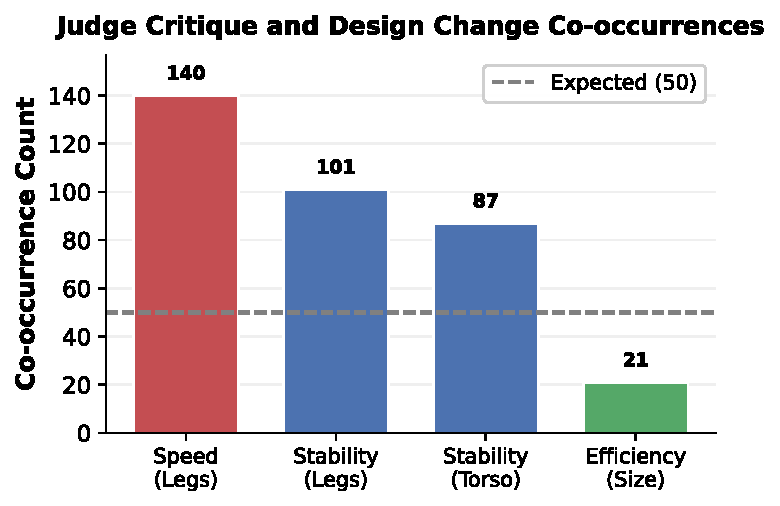
\includegraphics[width=0.7\linewidth]{figures/cooccurrence_bar_icml_outline.pdf}
\caption{Co-occurrence counts between judge critique types and design parameter changes. Dashed line indicates expected count under independence. All deviations are statistically significant ($p < 0.001$, $\chi^2$ test).}
\label{fig:cooccurrence}
\end{figure}

Additionally, we compared design change magnitudes between \abbrev{} runs and control runs without criterion-specific judges using Mann-Whitney U tests. \abbrev{} runs exhibited significantly smaller total change magnitudes ($0.126 \pm 0.102$ vs.\ $0.220 \pm 0.134$; $p = 0.001$) and leg geometry changes ($0.089 \pm 0.079$ vs.\ $0.172 \pm 0.124$; $p < 0.001$), suggesting that multi-objective feedback leads to more targeted, incremental refinements rather than large exploratory jumps.

\paragraph{Interpretation.}
These results provide evidence that the design agent responds to judge feedback in a topically coherent manner. Speed and stability critiques lead to locomotion-relevant parameter modifications, while efficiency concerns prompt different design strategies. The reduced change magnitudes in \abbrev{} runs suggest that criterion-specific judges help guide more focused exploration of the design space.

\paragraph{Caveat (missing objectives).}
In environments where a judge's target metric is not logged or is near-constant (e.g., stability for HalfCheetah and Swimmer in our current setup), that judge's critique may be less grounded, and its inclusion can dilute the usefulness of feedback for multi-objective search. This aligns with the 2D hypervolume behavior discussed in Section~\ref{sec:ablation_studies}.

\subsection{Example Debate Transcript}
\label{app:debate-transcript}

To illustrate the dialectical debate process, we present an example from an Ant run (seed 0 from the main experiments). This transcript shows rounds 0--2, where the score improved from 27,784 to 39,736 (+43\%).

\begin{figure}[htbp]
    \centering
    \begin{subfigure}[b]{0.32\textwidth}
        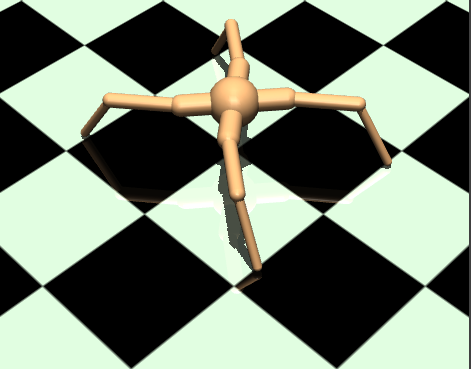
\includegraphics[width=\textwidth]{figures/round0.png}
        \caption{Round 0 (27,784)}
    \end{subfigure}
    \hfill
    \begin{subfigure}[b]{0.32\textwidth}
        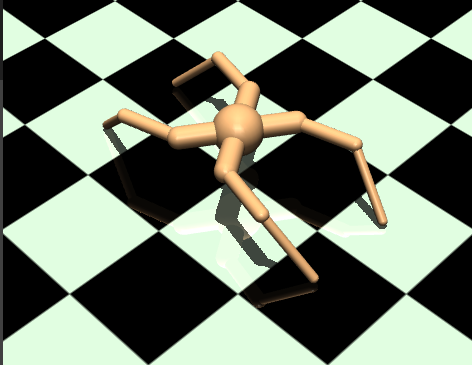
\includegraphics[width=\textwidth]{figures/round1.png}
        \caption{Round 1 (36,830)}
    \end{subfigure}
    \hfill
    \begin{subfigure}[b]{0.32\textwidth}
        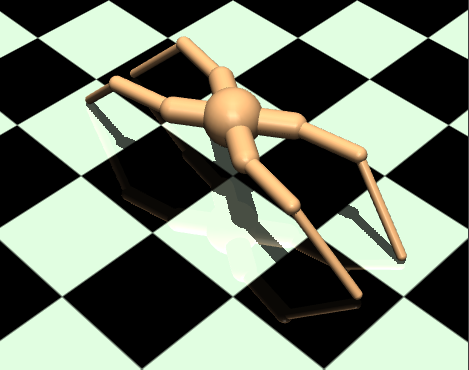
\includegraphics[width=\textwidth]{figures/round2.png}
        \caption{Round 2 (39,736)}
    \end{subfigure}
    \caption{Morphological progression over debate rounds (Ant, seed 0). Key changes: torso radius increases (0.14$\to$0.18), stance widens (0.22$\to$0.30), shin extends (0.34$\to$0.62). Score improves 43\% from round 0 to round 2.}
    \label{fig:debate-morphology}
\end{figure}

\paragraph{Round 0: Initial Synthesis.}
The design agent proposes an initial morphology:

\begin{promptbox}
A smaller torso with wider, more lateral leg attachments increases roll stability at speed, while thighs and shins are angled more downward than forward to reduce scuffing and allow higher step frequency. Slightly thicker proximal links keep robustness for ground impacts, with light distal links to minimize swing inertia for a fast trot.
\end{promptbox}

\noindent\textbf{Parameters:} torso=0.14, leg attachment=(0.22, 0.18), thigh=(0.24, 0.30), shin=(0.20, 0.34), capsule radii=(0.06, 0.04, 0.025).

\paragraph{Round 0: Control Agent Critique.}
The control agent identifies potential failure modes:

\begin{promptbox}
The smaller torso and light distal links may encourage very fast but bounce-prone gaits that amplify pitch/roll oscillations and foot scuffing, making the system fragile to impacts and contact-force spikes, prone to wasted energy from high-frequency action jitter, and harder to control at speed without explicit rewards for uprightness, smooth torques, adequate ground clearance, and moderated contact impulses.
\end{promptbox}

\paragraph{Round 0: Judge Panel Feedback.}
After simulation (\textbf{score: 27,784}), the criterion-specific judges provide feedback:

\begin{promptbox}
Speed: The morphology achieves sustained high forward translation, indicating an efficient gait that prioritizes speed while remaining stable enough to maintain continuous locomotion.

Stability: Despite strong travel distance, the design likely prioritizes speed over robustness, showing marginal upright stability with increased contact events and fall susceptibility under perturbations.

Efficiency: The very large travel distance over a moderate episode length suggests high average speed likely sustained by continuous torque, indicating potentially high energy-per-distance despite good task performance.

Novelty: The parameter pattern suggests a fairly balanced, near-symmetric morphology with only modest extremes, indicating limited structural distinctness.
\end{promptbox}

\paragraph{Round 1: Revised Design.}
Informed by the critique, the design agent proposes:

\begin{promptbox}
A slightly larger torso and thicker proximal links trade a bit of agility for much better pitch/roll damping at high speed, reducing bounce and contact spikes. Very long, mostly lateral thigh+shin segments act like compliant outriggers that enable an aggressive fast trot/bound with long effective stride while keeping distal mass low for quick swing.
\end{promptbox}

\noindent\textbf{Key parameter changes:}
\begin{itemize}[nosep,leftmargin=*]
    \item Increased torso radius (0.14 $\to$ 0.16) for better pitch/roll damping
    \item Wider leg attachment (0.22 $\to$ 0.30) for stability
    \item Longer shin segment (0.34 $\to$ 0.48) for increased stride length
    \item Thicker proximal capsule (0.06 $\to$ 0.07) for impact robustness
\end{itemize}

\noindent\textbf{Score: 36,830} (+33\% over round 0). The Speed judge notes: ``The morphology sustains fast, stable forward locomotion and greatly outpaces baseline distance.'' The Stability judge adds: ``The long episode duration and strong travel suggest sustained upright, stable locomotion with few destabilizing contacts.''

\paragraph{Round 2: Continued Improvement.}
The control agent critiques:

\begin{promptbox}
The current reward shaping risks over-optimizing raw forward velocity for this long-stride, low-distal-mass design, leading to pogo-stick vertical bounce, pitch/roll oscillations, high contact-force spikes, and action jitter that produce fragile high-speed gaits.
\end{promptbox}

\noindent The design agent responds:

\begin{promptbox}
Large torso with a very wide stance improves high-speed pitch/roll stability so the policy can push harder without tipping. Long, mostly lateral thigh plus longer shin increases effective stride length and ground contact leverage for fast trotting/bounding.
\end{promptbox}

\noindent\textbf{Key parameter changes:}
\begin{itemize}[nosep,leftmargin=*]
    \item Increased torso radius (0.16 $\to$ 0.18)
    \item Widened stance via Y-offset (0.20 $\to$ 0.30)
    \item Further extended shin (0.48 $\to$ 0.62)
\end{itemize}

\noindent\textbf{Final score: 39,736} (+8\% over round 1, +43\% over round 0). The Speed judge: ``This morphology sustains very high forward travel with stable, efficient propulsion.'' The Stability judge: ``Sustained upright locomotion with minimal instability is implied by the long episode duration and high reward.''

\paragraph{Summary.}
This transcript illustrates the core debate dynamics: (1) critiques identify concrete failure modes (bounce-prone gaits, pitch/roll oscillations); (2) the design agent responds with targeted parameter changes that address these concerns; (3) judge feedback validates improvements and surfaces new considerations; (4) iterative refinement yields a 43\% improvement over two rounds. The archive mechanism preserves the best design from round 2 for the final output.

\section{Evaluation Metric Analysis}
\label{app:metric-correlation}

We use a cumulative distance-from-origin metric $S = \sum_{t=0}^{T-1} d_t$ rather than standard MuJoCo episode returns for evaluation. This section provides empirical evidence that $S$ correlates strongly with standard returns, validating our metric choice.

\paragraph{Rationale.}
Standard MuJoCo rewards include method-specific shaping terms (alive bonuses, control penalties, contact costs) that vary across reward designs. Using these returns for ranking would conflate task performance with reward engineering choices. Our metric $S$ is reward-agnostic: it measures only how far the robot travels, providing a fair comparison across methods with different reward structures.

\paragraph{Correlation analysis.}
Figure~\ref{fig:metric_correlation} shows the relationship between $S$ (cumulative distance) and standard episode returns. To ensure balanced comparison, we subsample 1,200 runs per environment from the candidate pool. Table~\ref{tab:metric_correlation} reports Spearman rank correlations, which are robust to non-linear relationships.

\begin{figure}[htbp]
    \centering
    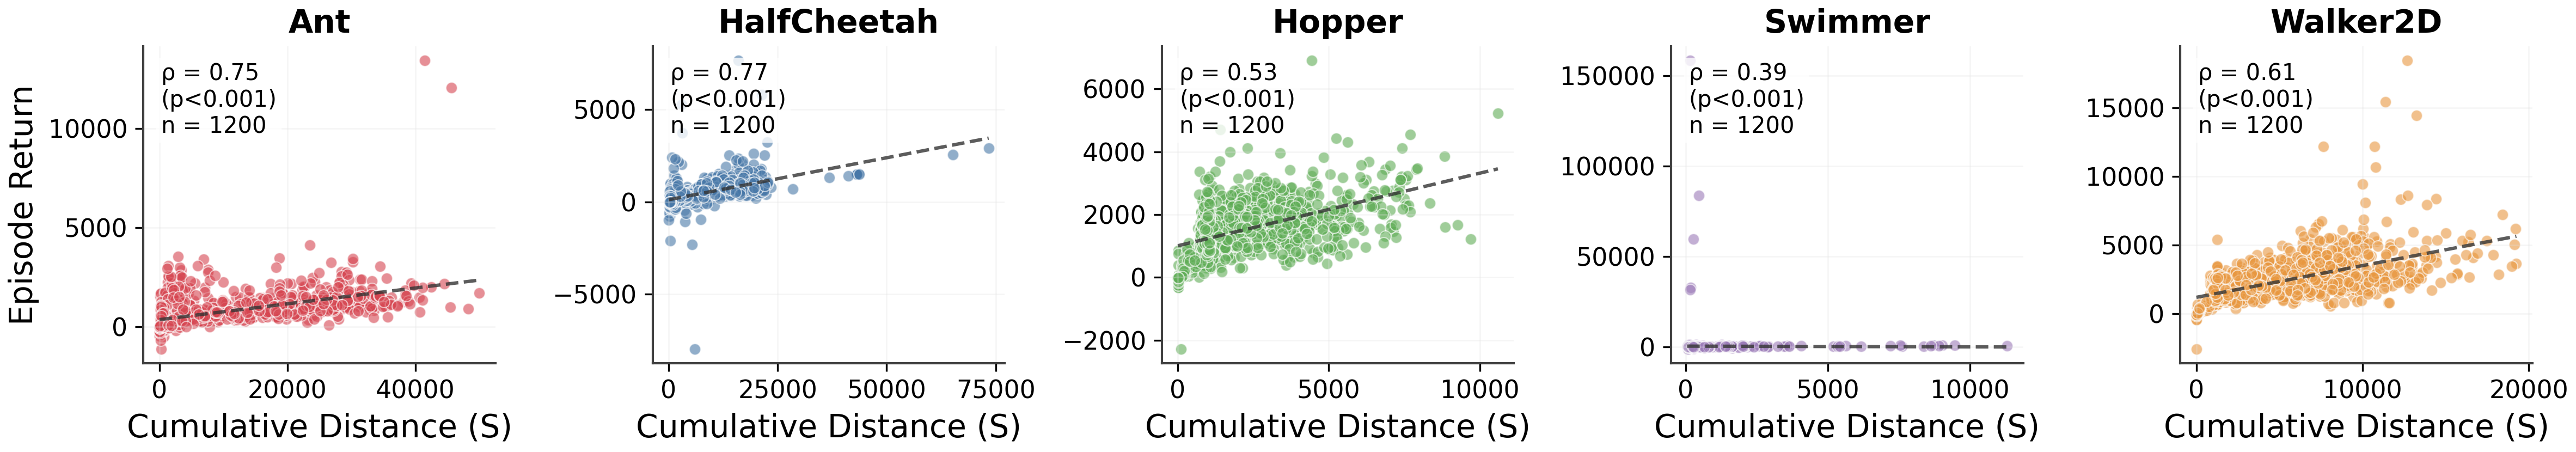
\includegraphics[width=\textwidth]{figures/metric_correlation.png}
    \caption{Correlation between cumulative distance metric $S$ and standard MuJoCo episode returns. Each point represents one training run. Dashed lines show linear regression fits. All correlations are statistically significant ($p < 0.001$).}
    \label{fig:metric_correlation}
\end{figure}

\begin{table}[htbp]
\centering
\caption{Correlation between cumulative distance $S$ and standard episode returns. Spearman $\rho$ measures rank correlation (robust to non-linearities). All correlations are statistically significant ($p < 0.001$).}
\label{tab:metric_correlation}
\small
\begin{tabular}{lccc}
\toprule
\textbf{Environment} & \textbf{N} & \textbf{Pearson $r$} & \textbf{Spearman $\rho$} \\
\midrule
Ant & 1,200 & 0.53 & 0.75 \\
HalfCheetah & 1,200 & 0.58 & 0.77 \\
Hopper & 1,200 & 0.51 & 0.53 \\
Swimmer & 1,200 & $-$0.01 & 0.39 \\
Walker2D & 1,200 & 0.57 & 0.61 \\
\midrule
\textbf{Mean} & 6,000 & --- & \textbf{0.61} \\
\bottomrule
\end{tabular}
\end{table}

\paragraph{Interpretation.}
The mean Spearman correlation of $\rho = 0.61$ indicates that $S$ and standard returns share substantial rank agreement: designs that score well on $S$ generally also achieve high episode returns. The moderate (rather than perfect) correlation is expected: standard returns include method-specific shaping terms (alive bonuses, control penalties) that $S$ intentionally excludes to isolate locomotion performance. The weaker Pearson correlation for Swimmer ($r = -0.01$) reflects a non-linear relationship in that environment, but the positive Spearman correlation ($\rho = 0.39$) confirms that higher $S$ still corresponds to better-ranked performance. These results demonstrate that our metric choice does not systematically bias results away from standard benchmarks while providing a fairer comparison across methods with different reward structures.

\paragraph{Ranking agreement for top candidates.}
Table~\ref{tab:ranking_agreement} provides additional evidence that selecting by $S$ does not sacrifice standard return performance. For each environment, we identify the best candidate by $S$ and report its percentile rank in terms of standard episode return. The best-$S$ candidate achieves a mean return percentile of 96.9\%, indicating it typically ranks in the top 3\% by standard returns. This confirms that $S$-based selection identifies high-quality designs under both metrics.

\begin{table}[htbp]
\centering
\caption{Ranking agreement between $S$ and standard returns. ``Return Percentile'' indicates where the best-$S$ candidate ranks in terms of episode return (higher = better). The best-$S$ candidate is typically in the top 3\% by standard returns.}
\label{tab:ranking_agreement}
\small
\begin{tabular}{lcc}
\toprule
\textbf{Environment} & \textbf{Return Percentile} & \textbf{Top-10 Overlap} \\
\midrule
Ant & 100.0\% & 1/10 \\
HalfCheetah & 99.9\% & 3/10 \\
Hopper & 99.9\% & 1/10 \\
Swimmer & 98.2\% & 0/10 \\
Walker2D & 86.6\% & 0/10 \\
\midrule
\textbf{Mean} & \textbf{96.9\%} & 1.0/10 \\
\bottomrule
\end{tabular}
\end{table}

\section{LLM Backbone Sensitivity}
\label{app:llm-sensitivity}

To assess whether \abbrev{}'s performance depends on LLM scale, we evaluated three OpenAI model variants on Ant: GPT-5-nano, GPT-5-mini, and GPT-5.2 (used in main experiments). Each configuration ran for 5 debate rounds with 3 seeds.

\paragraph{Final performance.}
Table~\ref{tab:llm_sensitivity} reports the best archived scores (normalized to the Default baseline). All three models achieve comparable final performance, with no statistically significant differences (pairwise t-tests, $p > 0.19$). This suggests \abbrev{}'s gains stem from the debate framework structure rather than raw model capability.

\begin{table}[htbp]
\centering
\caption{LLM backbone comparison on Ant (3 seeds $\times$ 80 candidates = 240 total per model). Normalized scores use the best archived result per seed. ``Degenerate'' counts candidates producing failed design--reward pairs (score $<100$ or invalid). Differences in final normalized scores are not statistically significant ($p > 0.19$).}
\label{tab:llm_sensitivity}
\small
\begin{tabular}{lcc}
\toprule
\textbf{Model} & \textbf{Norm. Score} & \textbf{Degenerate} \\
\midrule
GPT-5-nano & $3.60 \pm 0.26$ & 35.2\% \\
GPT-5-mini & $3.23 \pm 0.32$ & 49.2\% \\
\rowcolor{gray!15}
GPT-5.2 (main) & $3.18 \pm 0.28$ & 15.8\% \\
\bottomrule
\end{tabular}
\end{table}

\paragraph{Robustness differences.}
While final archived scores are comparable (due to the archive mechanism retaining the best candidate), smaller models produce substantially more degenerate candidates during the search process. GPT-5-mini has the highest failure rate (49.2\% of candidates produce near-zero scores), followed by GPT-5-nano (35.2\%). In contrast, GPT-5.2 achieves only 15.8\% degenerate candidates. These failures represent wasted computation: each candidate requires a full RL training run before the score reveals the design was defective.

\paragraph{Practical implications.}
The archive mechanism makes \abbrev{} robust to individual candidate failures, allowing final performance to remain comparable across model scales. However, smaller models require evaluating more candidates to find viable designs, increasing compute costs. We used GPT-5.2 for main experiments as it provides the most reliable code generation with fewer degenerate outputs per round.

\section{Open-Weight Backbone Analysis}
\label{app:open_weight_backbones}

To assess whether \abbrev{} depends on a proprietary frontier model, we reran the full pipeline with two DeepSeek open-weight backbones on Ant and Swimmer. Each run uses the same protocol as the main experiments: 3 search seeds, 5 debate rounds, 80 trained candidates per seed, identical RL hyperparameters, and the same Default-normalized evaluation score. We compare against GPT-5.2, the backbone used in the main experiments.

\begin{table}[H]
\centering
\caption{Open-weight backbone comparison under the same \abbrev{} protocol. Scores are Default-normalized best archived scores over 3 search seeds. DeepSeek-R1 retains $78\%$ of GPT-5.2 performance on Ant and $71\%$ on Swimmer; DeepSeek-V3 remains above the Default baseline on both tasks.}
\label{tab:open_weight_backbones}
\small
\setlength{\tabcolsep}{5pt}
\begin{tabular}{lccc}
\toprule
\textbf{Backbone} & \textbf{Access} & \textbf{Ant} & \textbf{Swimmer} \\
\midrule
GPT-5.2 & Proprietary & $3.18$ & $9.35$ \\
DeepSeek-R1 & Open-weight & $2.47$ & $6.62$ \\
DeepSeek-V3 & Open-weight & $1.85$ & $3.72$ \\
\bottomrule
\end{tabular}
\end{table}

The open-weight models do not match GPT-5.2, but both remain above the Default baseline on the two tested environments. The stronger DeepSeek-R1 result is consistent with \abbrev{} benefiting from explicit reasoning during critique and synthesis. The DeepSeek-V3 result is still useful: even without a reasoning trace, the debate loop produces viable design--reward pairs rather than collapsing to default-level performance. These experiments support the conclusion that \abbrev{} is not tied to a single proprietary backbone, although model capability affects sample efficiency and final score.
